\chapter{Virtual Functions and Late Bindings}
\section{Programmazione orientata agli oggetti}
La programmazione ad oggetti è diversa ad altri tipi di programmazione (tipo askle che è un linguaggio funzionale, o l'approccio imperativo, ovvero  un approccio in cui si dice al computer cosa fare passo passo attraveroso un a serie di comandi) è quella di rappresentare un mondo un cui degli elementi (oggetti) interagiscono tra di loro. \\

La programmazione ad oggetti è diversa ad altri tipi di programmazione (tipo askle che è un linguaggio funzionale, o l'approccio imperativo, ovvero  un approccio in cui si dice al computer cosa fare passo passo attraveroso un a serie di comandi) è quella di rappresentare un mondo un cui degli elementi (oggetti) interagiscono tra di loro. \\

Alcuni concetti fondamentali della programmazione ad oggetti sono:
\begin{itemize}
    \item \textbf{Classe}: è un modello, uno schema, una struttura che definisce le proprietà e i comportamenti comuni degli oggetti di quel tipo. Una classe può essere vista come un "progetto" o un "blueprint" per creare oggetti
    \item \textbf{Ereditarietà}: è un meccanismo che consente a una classe di ereditare le proprietà e i comportamenti di un'altra classe. La classe che eredita è chiamata "classe derivata" o "sottoclasse", mentre la classe da cui si eredita è chiamata "classe base" o "superclasse". L'ereditarietà permette di creare gerarchie di classi e di riutilizzare il codice.
    \item \textbf{Polimorfismo}: è la capacità di un oggetto di assumere diverse forme o comportamenti a seconda del contesto in cui viene utilizzato. In altre parole, il polimorfismo consente a un oggetto di essere trattato come un'istanza di una classe base, ma di eseguire il comportamento specifico della sua classe derivata. Si divide in:
    \begin{itemize}
        \item \textbf{Polimorfismo ad hoc}: si riferisce alla capacità di una funzione o di un metodo di avere lo stesso nome ma comportarsi in modo diverso a seconda del tipo o del numero di argomenti passati. Questo è spesso realizzato attraverso l'overloading dei metodi.
        \item \textbf{Polimorfismo di sottotipo}: ovvero la capacità di un oggetto di una classe derivata di essere trattato come un'istanza della sua classe base. Questo è spesso realizzato attraverso l'overriding dei metodi.
        \item \textbf{Polimorfismo parametrico}: si riferisce alla capacità di una funzione o di un metodo di operare su tipi generici, consentendo di scrivere codice che può essere riutilizzato con diversi tipi di dati. Questo è spesso realizzato attraverso l'uso di generics o template. Ad esempio
    \end{itemize}
\end{itemize}
\section{Funzioni virtuali}
\dfn{Funzione virtuale}{
    una funzione si definisce virtuale un metdo non statico di una classe base che può essere \textbf{ridefinita} (overridden) in una classe derivata
}


\subsection{Overriding}
\dfn{Overriding}{
    l'ovverinding è la metodologia tramite la quale vado a sostiuire il corpo di un metodo con uno nuovo a runtime    
}

l'overriding si applica in tali circostanze:
\begin{itemize}
    \item il metodo overridden è una funzione virtuale
    \item la funzione nella classe derivata ha la stessa signature della funzione nella classe base
\end{itemize}

Si ricorda che la \textbf{signature} di una funzione è composta da:
\begin{itemize}
    \item Nome della funzione
    \item parametri formali
    \item numero di parametri formali
    \item il \textit{tipo di ritorno} non fa parte della signature
\end{itemize}

La signature di una funzione con il suo \textit{tipo di ritorno} è detta \textbf{prototipo} della funzione. \\
I metodi statici non posso no essere sottoposti a overriding in quanto non sono associati ad un'istanza della classe ma alla classe stessa. se si dichiara, inoltre, nella classe derivata una funzione con la stessa signature ma con un tipo diverso il compilatore restituirà errore. In c++ se io dichiaro una classe derivata con lo stesso nome cma con una signature io precludo la visita della funzione della classe base. Si noti tale affermazione:

\nt{
    Quando si invoca una funzione virtuale per un oggetto il cui tipo è conosciuto a tempo di compilazione, il comportamento della funzione, dal punto di vista dell'utente, è lo stesso di quello di una funzione non virtuale. 
}

\mprop{sulle funzioni virtuali}{
    Quando una funzione virtuale $f$ è  invocata per un oggetto $o$ della classe $D$ derivata da $B$ ci snoo tre possibilità:
    \begin{itemize}
        \item $f$ è definita solo in $D$: viene invocata la versione di $D.f$ da $o$
        \item $f$ è definita solo in $B$: viene invocata la versione di $B.f$ da $o$
        \item $f$ è definita sia in $B$ che in $D$: viene invocata la versione di $D.f$ da $o$
    \end{itemize}
}

il vantaggio è che quando di usare funzioni  è quello di manipolare gli oggetti tramite riferimenti o puntatori alla classe base. In questo modo, è possibile scrivere codice più generico e riutilizzabile, poiché non è necessario conoscere il tipo esatto dell'oggetto a cui si sta facendo riferimento.

\subsubsection{Esempi}

\begin{lstlisting}[language=C++]
class B {
    public:
        virtual void f() { cout << "B::f" << endl; } // funzione virtuale
};

class D : public B {
    public:
        void f() override { cout << "D::f" << endl; } // overriding della funzione virtuale
};
int main() {
    B* b = new B();
    B* d = new D();

    b->f(); // Output: B::f
    d->f(); // Output: D::f (polimorfismo in azione)

    delete b;
    delete d;
    return 0;
}
\end{lstlisting}

\subsubsection{Funzioni virtuali in Java e C++}
\paragraph{Java}
in Javam tutti i metodi non statici sono virtuali di default, quindi non è necessario dichiararli esplicitamente come virtuali. Tuttavia, è possibile utilizzare la parola chiave \texttt{final} per impedire che un metodo venga sovrascritto in una sottoclasse. ad esempio
\begin{lstlisting}[language=Java]
class B {
    public void f() { System.out.println("B::f"); } // funzione virtuale
}
class D extends B {
    @Override
    public void f() { System.out.println("D::f"); } // overriding della funzione virtuale
}
public class Main {
    public static void main(String[] args) {
        B b = new B();
        B d = new D();
        b.f(); // Output: B::f
        d.f(); // Output: D::f (polimorfismo in azione)
    }
}
\end{lstlisting}
\paragraph{C++}
in C++ le funzioni non sono virtuali di default, quindi è necessario dichiararle esplicitamente come virtuali utilizzando la parola chiave \texttt{virtual}. Ad esempio
\begin{lstlisting}[language=C++]
class B {
    public:
        virtual void f() { cout << "B::f" << endl; } // funzione virtuale
};  
class D : public B {
    public:
        void f() override { cout << "D::f" << endl; } // overriding della funzione virtuale
};
int main() {
    B* b = new B();
    B* d = new D();
    b->f(); // Output: B::f
    d->f(); // Output: D::f (polimorfismo in azione)
    delete b;
    delete d;
    return 0;
}
\end{lstlisting}
\subsection{Early binding}
\dfn{Early binding}{
    l'early binding è il processo di associazione di una chiamata a funzione con la sua definizione durante la fase di compilazione del programma
}

It's the method used by most non OO languages, and it's also the default behaviour for functions and methods in C++ (if not declared as virtual). 

\subsection{Late binding}
\dfn{Late binding}{
    The correct address of the code to execute after a funciton call is deduced only at runtime.
}

Late binding can be implemented by simply using a VTABLE, or a table of virtual function pointers relative to each class:

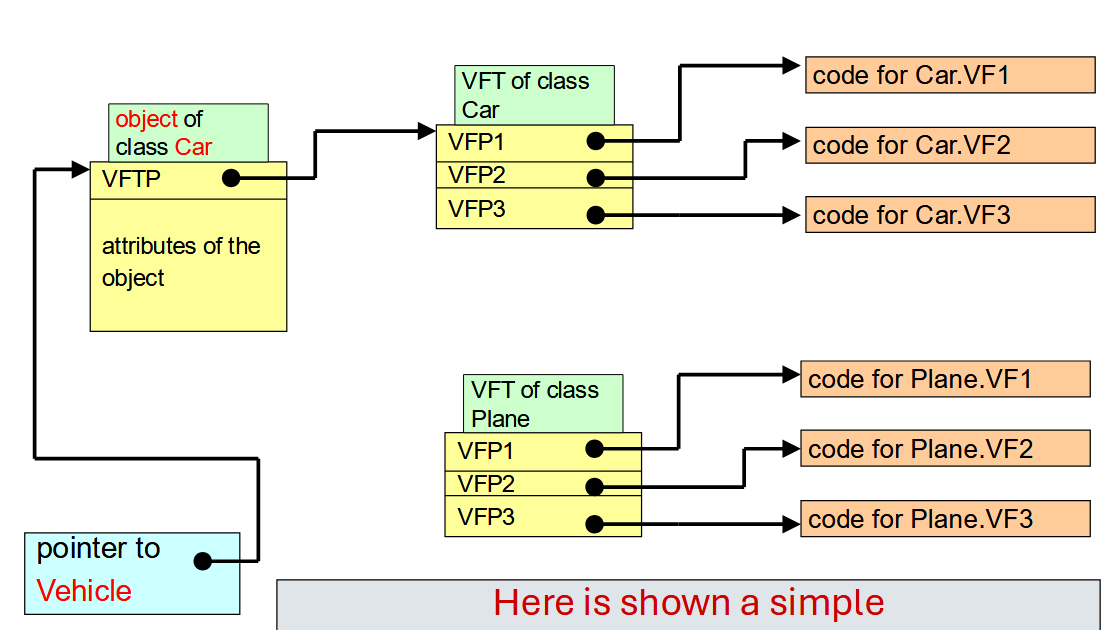
\includegraphics[width=0.5\textwidth]{img/implLateBinding.png}

Each object has a hidden pointer to the virtual funciton table (VTABLE) of it's class.

In short, the following steps are performed for every virtual funcion call:
\begin{enumerate}
    \item The program looks for the VFTP in the object
    \item It then searches the table for the correct VFP using the funciton name
    \item If the pointer is found, the code pointed to is executed
\end{enumerate}

The reason why not all function calls are virtual in most languages is because of eficiency, although in most cases the overhead generated by virtualization is negligible.

\section{Examples}
\begin{lstlisting}[language=C++]
#include <iostream>
#include <string>
void prn( std::string s) {
    std::cout << s << "\n";
}
class A {
  public:
    virtual void f() { prn("A::f()"); }
    void g() { prn("A::g()"); }
    virtual void h() { prn("A::h()"); }
    void i() { prn("A::i()"); }
};
class B : public A {
  public:
    virtual void f() { prn("B::f()"); }
    virtual void g() { prn("B::g()"); }
    void h() { prn("B::h()"); }
    void i() { prn("B::i()"); }
};
class C : public B{
  public:
    virtual void f() { prn("C::f()"); }
    void g() { prn("C::g()"); }
    void h() { prn("C::h()"); }
    void i() { prn("C::i()"); }
};
class D : public A {
  public:
    virtual void h() { prn("D::h()"); }
    void m() {
        prn("D::m()");
        h();
    }
    virtual void g() { prn("D::g()"); }
};
class E : public D {
  public:
    virtual void f() { prn("E::f()"); }
    virtual void h() { prn("E::h()"); }
    void i() {
        prn("E::i()");
        m();
    }
    void g() { prn("E::g()"); }
};
class G : public E {
  public:
    virtual void f(int i) { prn("G::f(int)"); }
};

int main() {
    A anA;
    A *a;
    B aB;
    B *b;
    a = new B();
    a->f();
    a->g();
    b = (B*)a;
    b->f();
    b->g();
    A &arA = *new E();
    arA.i();
    E anE;
    anE.i();
    arA.g();
    D *apD = &anE;
    apD->g();
    A *apA = &anE;
    apA->g();
    G aG;
    aG.f();
    aG.f(3);
    aG.h();
    aG.i();
    aG.g();
    a = &aG;
    a->f();
    a->f(3);
    a->h();
    a->i();
    a->g();
    G *pG;
    pG = (G*)a;
    pG->f();
    pG->f(3);
    pG->h();
    pG->i();
    pG->g();
}
\end{lstlisting}

Given the C++ classes defined above, here are some interesting function calls to look at:
\begin{itemize}
    \item a->f(): at runtime, a is a pointer to an object of class B. Seen as f is declared virtual in A it is overridden by the B class and "B::f()" is output.
    \item a->g(): because g is not declared as virtual in A, early binding is used and the function declared in A is used and "A::g()" is output.
    \item aG->f(): a function with signature f() is decalred in class G's superclass (E), but G also defines a function with name f but with a different signature (f(int)). Thus the homonymous function in the superclass is hidden and an error occurs.
    \item a = \&aG; a->f(): f() is virtual in A, so late binding is used. f(int) is defined in G but its signatura doesn't match, so E's definition for f() is used instead.
    \item a = \&aG; a->f(int): because A doesn't have any definition for a function with signature f(int), an error is thrown.
\end{itemize}